\documentclass[border=10pt]{standalone}
\usepackage{pgfplots}
\pgfplotsset{compat=1.18}
\usetikzlibrary{arrows.meta}
\usepgfplotslibrary{fillbetween}

\begin{document}
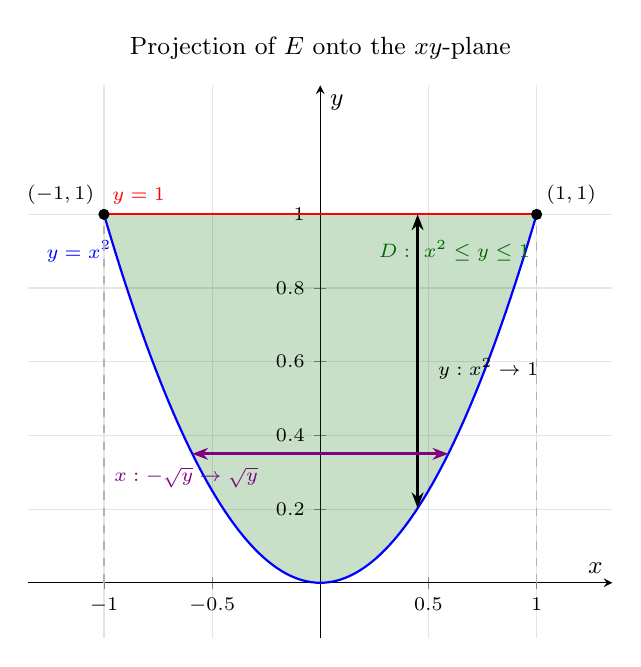
\begin{tikzpicture}
\begin{axis}[
    width=9cm, height=8.6cm,
    xmin=-1.35,xmax=1.35, ymin=-0.15,ymax=1.35,
    axis lines=middle,
    xlabel=$x$, ylabel=$y$,
    xtick={-1,-0.5,0.5,1}, ytick={0.2,0.4,0.6,0.8,1},
    tick label style={font=\scriptsize}, label style={font=\small},
    title={Projection of $E$ onto the $xy$-plane},
    title style={font=\small},
    grid=major, grid style={gray!20},
]

% ---- visible, named boundary curves ----
\addplot[thick, blue, name path=parab, domain=-1:1, samples=101] {x^2}
    node[pos=0.06, above left, font=\scriptsize, text=blue] {$y=x^2$};
\addplot[thick, red, name path=top, domain=-1:1, samples=2] {1}
    node[pos=0.08, above, font=\scriptsize, text=red] {$y=1$};

% ---- shaded base region D :  x^2 <= y <= 1 ----
\addplot[green!45!black, opacity=0.22, draw=none] fill between[of=top and parab];
\node[font=\scriptsize, green!40!black, anchor=center] at (axis cs:0.62,0.9)
    {$D:\ x^2\le y\le 1$};

\draw[dashed, gray!60] (axis cs:-1,0) -- (axis cs:-1,1);
\draw[dashed, gray!60] (axis cs:1,0)  -- (axis cs:1,1);
\addplot+[only marks, mark=*, mark size=1.8, black] coordinates {(-1,1) (1,1)};
\node[font=\scriptsize, anchor=south east] at (axis cs:-1,1) {$(-1,1)$};
\node[font=\scriptsize, anchor=south west] at (axis cs:1,1) {$(1,1)$};

% ---- typical vertical strip:  y from x^2 to 1 ----
\draw[{Stealth[length=2mm]}-{Stealth[length=2mm]}, very thick, black]
    (axis cs:0.45,{0.45^2}) -- (axis cs:0.45,1);
\node[font=\scriptsize, anchor=west] at (axis cs:0.5,0.58) {$y:x^2\to 1$};

% ---- typical horizontal strip:  x from -sqrt(y) to sqrt(y) ----
\draw[{Stealth[length=2mm]}-{Stealth[length=2mm]}, very thick, violet]
    (axis cs:{-sqrt(0.35)},0.35) -- (axis cs:{sqrt(0.35)},0.35);
\node[font=\scriptsize, anchor=north, violet] at (axis cs:-0.62,0.34)
    {$x:-\sqrt{y}\to\sqrt{y}$};
\end{axis}
\end{tikzpicture}
\end{document}
